% \section{Introduction}

% On-policy distillation (OPD) \cite{agarwal2024onpolicydistillationlanguagemodels, gu2026minillmonpolicydistillationlarge} is a knowledge distillation method for large language models (LLMs) that trains the student on trajectories sampled from its own policy, while using teacher feedback to provide dense token-level supervision on the on-policy rollouts. A particularly important branch of OPD is on-policy self-distillation (OPSD), where the teacher and the student are derived from the same base model under different contexts. The student generates trajectories using the original context, while the teacher is constructed by exposing the same model to privileged information, such as ground-truth solutions or environment feedback. Instead of relying on an external stronger teacher, OPSD converts training-time information into dense supervision that can be distilled back into the model itself. Compared with reinforcement learning with verifiable rewards (RLVR) \cite{tu2025positionhiddencostsmeasurement, wang2025reinforcementlearningreasoninglarge, lambert2025tulu3pushingfrontiers}, this supervision is more sample efficient, and less prone to catastrophic forgetting during post-training \cite{shenfeld2026selfdistillationenablescontinuallearning, zhao2026selfdistilledreasoneronpolicyselfdistillation}.

% Recent work show that OPSD is effective in several applications. It has been used to internalize richer contexts or system prompts into the model behavior \cite{ye2026onpolicycontextdistillationlanguage, sang2026onpolicyselfdistillationreasoningcompression}, to acquire domain knowledge and maintain capabilities during continual adaptation \cite{shenfeld2026selfdistillationenablescontinuallearning, hubotter2026reinforcementlearningselfdistillation}, and to improve preference alignment \cite{wang2026openclawrltrainagentsimply}.

% Despite these promising results, our understanding of OPSD remains fragmented. Existing work differs in many dimensions, including what privileged information is exposed, whether the teacher is fixed or changing, and which optimization objective is used. As a result, researchers lack a clear design guide for when OPSD should help and which design choices matter.

% This gap is especially important because recent studies now report conflicting conclusions about OPSD on reasoning tasks. Earlier work suggests that OPSD can improve mathematical reasoning and related capabilities \cite{zhao2026selfdistilledreasoneronpolicyselfdistillation, ye2026onpolicycontextdistillationlanguage}. In contrast, newer studies show that its behavior can be unstable, and in some cases self-distillation can noticeably degrade reasoning performance \cite{fu2026revisitingonpolicydistillationempirical, kim2026doesselfdistillationsometimesdegrade}. 
% For example, Fu et al. \cite{fu2026revisitingonpolicydistillationempirical} argues that sampled-token OPSD objectives are fragile because they reduce a distribution-level matching problem to an imbalanced one-token signal. \cite{fu2026revisitingonpolicydistillationempirical} Another shows that richer privileged information can suppress the model's expression of uncertainty during reasoning. \cite{kim2026doesselfdistillationsometimesdegrade} Together, they suggest that OPSD's performance in reasoning tasks is unstable.



\section{Introduction}

\begin{figure}[!t]
  \centering
  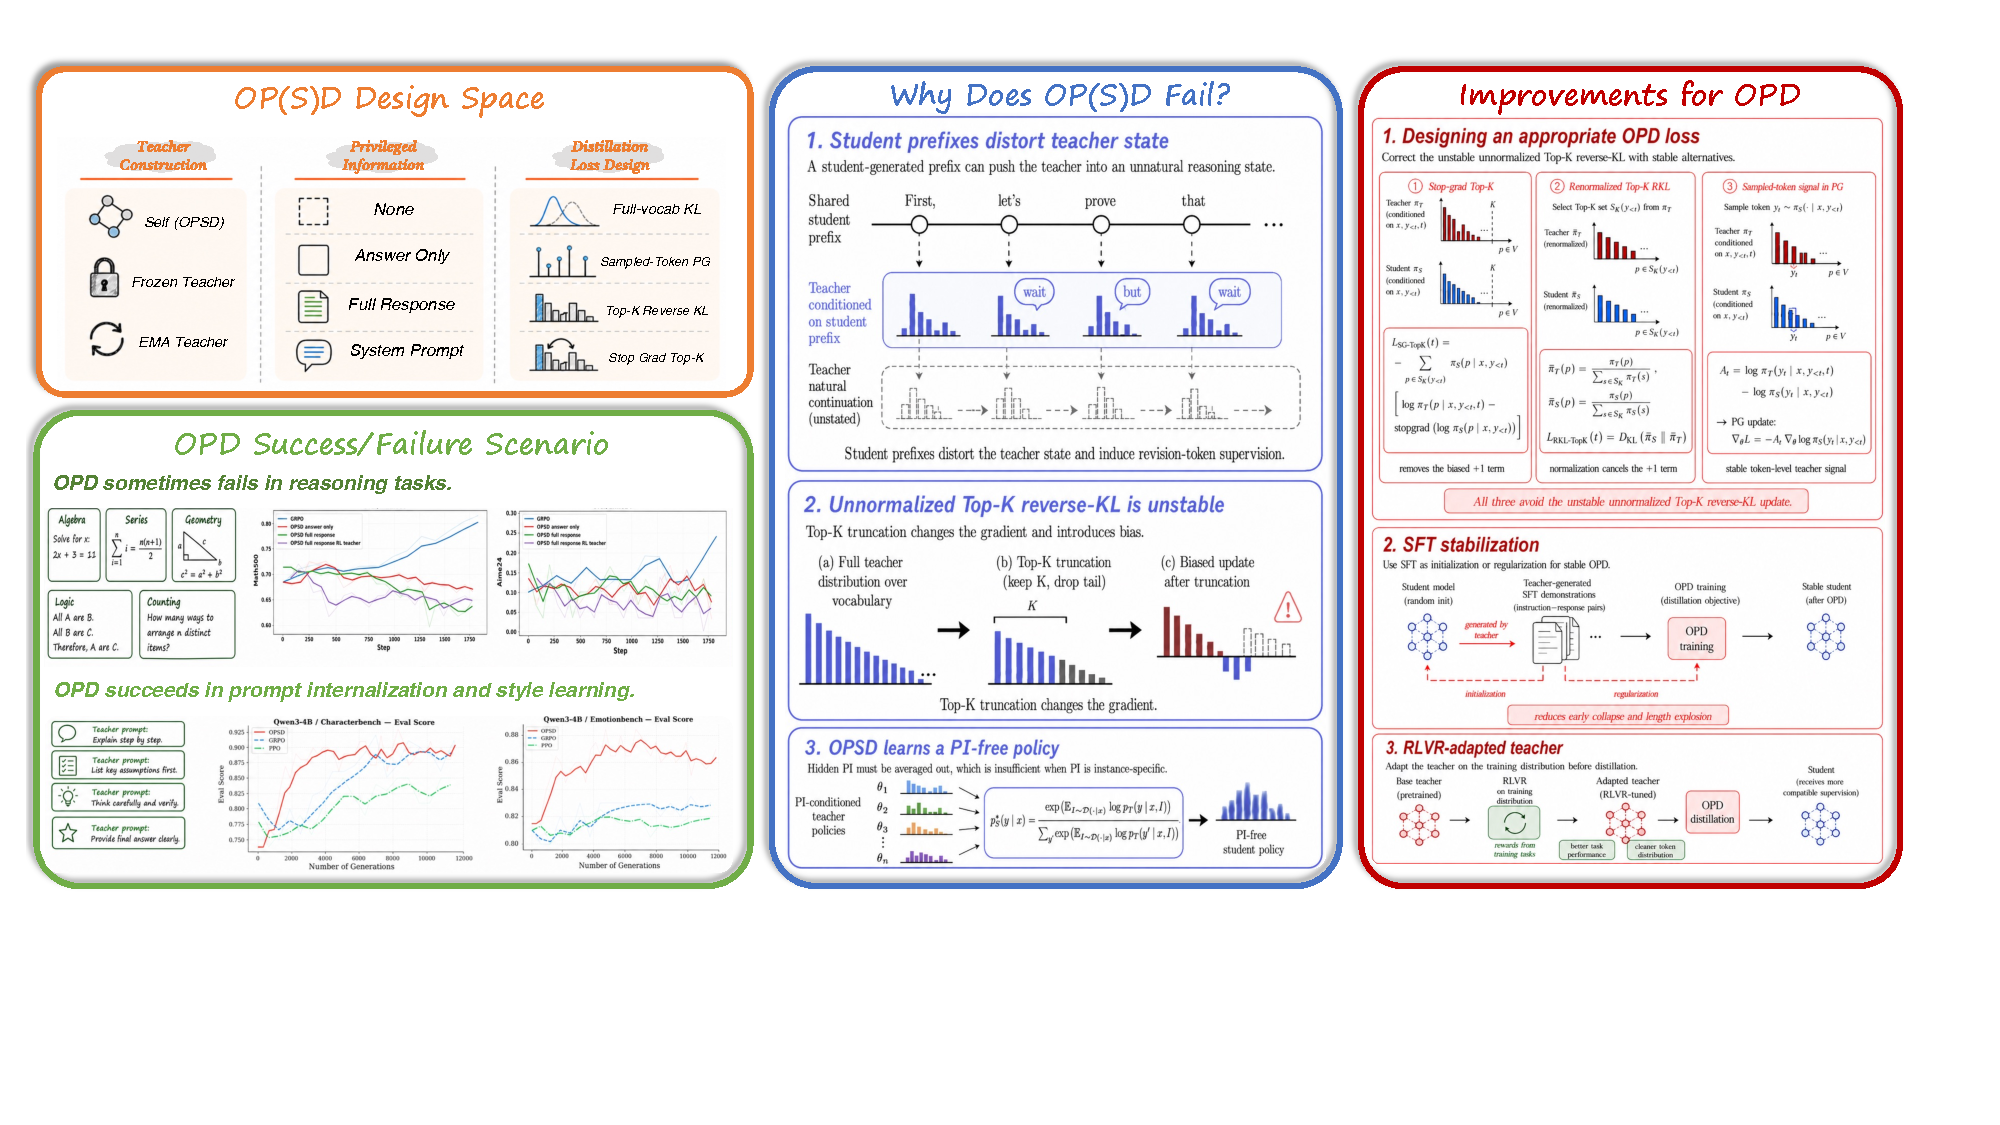
\includegraphics[width=\textwidth]{figures/overview.pdf}
  \caption{
    \textbf{Overview.} We map the OP(S)D \emph{design space} (left, top) and its task-dependent success/failure behavior (left, bottom), identify three failure mechanisms—prefix-distorted teacher state, biased Top-$K$ reverse-KL, and PI-marginalized OPSD policy (middle), and propose practical fixes: stable Top-$K$ losses, SFT stabilization, and RLVR-adapted teachers (right).
  }
  \label{fig:overview}
\end{figure}

On-policy distillation (OPD) \cite{agarwal2024onpolicydistillationlanguagemodels, gu2026minillmonpolicydistillationlarge} is a promising post-training
algorithm for large language models (LLMs). Instead of training on off-policy responses, OPD trains the student on trajectories sampled from
its own policy and uses one or more teacher models to provide dense token-level supervision
along these on-policy rollouts. This makes OPD appealing as a practical mechanism
for integrating the capabilities of multiple stronger teachers into the student \cite{deepseekai2026deepseekv4, coreteam2026mimov2flashtechnicalreport}, mitigating
catastrophic forgetting, and improving sample efficiency \cite{lu2025onpolicydistillation, shenfeld2026selfdistillationenablescontinuallearning}. A closely related topic is on-policy self-distillation (OPSD), where the teacher is not a stronger model but the student model itself conditioned on
additional privileged information (PI) \cite{zhao2026selfdistilledreasoneronpolicyselfdistillation, sang2026onpolicyselfdistillationreasoningcompression,ye2026onpolicycontextdistillationlanguage}. The PI may include ground-truth answers, system prompts or user preferences. These methods are attractive for post-training because they can convert teacher behavior or training-time context into supervision on the student’s own state distribution.





Despite the conceptual simplicity, the empirical behavior of OPD and OPSD remains
poorly understood. Prior work has reported successful applications of
self-distillation for context internalization and reasoning \cite{zhao2026selfdistilledreasoneronpolicyselfdistillation, sang2026onpolicyselfdistillationreasoningcompression, ye2026onpolicycontextdistillationlanguage}. However, recent studies argue that
on-policy (self) distillation can be unstable and may degrade
performance \cite{fu2026revisitingonpolicydistillationempirical,  kim2026doesselfdistillationsometimesdegrade}. These mixed results raise a basic question: \textbf{when do OPD and OPSD
actually work, when do they fail, and what mechanisms explain the difference}?

In this paper, we present a comprehensive empirical study of OPD and OPSD across
both successful and failing regimes. On reasoning tasks, OPD provides only
conditional benefits and can suffer from length explosion, repetition, and
teacher-student mismatch, while OPSD fails in our tested math reasoning
settings. In contrast, OPSD is effective for system-prompt internalization and
alignment, where the privileged information induces a shared latent behavior that can be compressed into a PI-free policy at test time.

We identify three mechanisms behind these outcomes. First, student-generated
prefixes can move the teacher into states where its token-level supervision is
locally incompatible with the student's trajectory. Second, Top-$K$ reverse-KL
approximations can introduce biased gradients and destabilize optimization. Third, OPSD only learns a single PI-free consensus policy across PI-conditioned teachers, which is insufficient when PI is instance-specific.

Motivated by these findings, we study practical stabilizers for OPD: a
stop-gradient Top-$K$ KL surrogate that removes the biased gradient term, Reinforcement Learning with Verifiable Rewards (RLVR)
adaptation of the teacher to improve task performance, and Supervised Fine-Tuning (SFT) the student to improve output format and stabilize response-length dynamics.

Our contributions are:
\begin{itemize}
    \item We empirically study when OPD and OPSD succeed or fail in reasoning, system-prompt internalization, and alignment. \item We identify three failure mechanisms: prefix-induced teacher-student mismatch, biased TopK reverse-KL gradients, and OPSD's PI-free aggregation across instance-specific PI. 
    \item We propose practical stabilizers based on stop-gradient Top-$K$ KL,
    RLVR-adapted teachers, and student SFT for output well-formedness
    and response length stabilization.
\end{itemize}

